\documentclass[skip,a4paper]{article}

\usepackage{ucs}
\usepackage[utf8x]{inputenc}
\usepackage[T1]{fontenc}
\usepackage{amsmath}
\usepackage{amsfonts}
\usepackage{amssymb}
\usepackage[top=1cm,bottom=1cm,right=2cm,left=1cm]{geometry}
\usepackage{titlesec}
\usepackage{array}
\usepackage{enumitem}
%% URLs
\usepackage{hyperref}
\usepackage{url}
\usepackage{ulem} % em is underlined

%% Graphics and colors
\usepackage{tikz} % Round corner on picture
\usepackage{color} % enable color
\usepackage{xcolor} % Define own colors
\usepackage{graphicx} % Include picts.

%% Fonts
% cf http://www.tug.dk/FontCatalogue/seriffonts.html
\usepackage[default,osfigures,scale=0.95]{opensans}
% Symbols
\usepackage{marvosym}


%-----Liens PDF-----%
\hypersetup{
	%backref=true, %permet d'ajouter des liens dans...
	%pagebackref=true,%...les bibliographies
	%hyperindex=true, %ajoute des liens dans les index.
	colorlinks=true, %colorise les liens
	breaklinks=true, %permet le retour à la ligne dans les liens trop longs
	urlcolor=black, %couleur des hyperliens
	linkcolor=black, %couleur des liens internes
	%bookmarks=true, %créé des signets pour Acrobat
	%bookmarksopen=true, %si les signets Acrobat sont créés,
	%les afficher complètement.
	pdftitle={\title}, %informations apparaissant dans
	pdfauthor={\author}, %dans les informations du document
	pdfsubject={\subject} %sous Acrobat.
}

\makeatletter

\pagestyle{empty}

\def\UrlFont{\em} % url are `em`, and `em` is underlined with ulem

\titleformat{\section}{\LARGE\bfseries\color{redcv}}{\thesection}{1em}{}[{\titlerule[0.8pt]}]
\titleformat{\subsection}{\normalfont\Large\bfseries}{\thesubsection}{1em}{}

\titlespacing*{\section}{0pt}{2ex plus 0.4ex minus .2ex}{1.3ex plus .2ex}
\titlespacing*{\subsection}{50pt}{2ex plus 0.4ex minus -0.2ex}{0.5ex plus .2ex}

\newcommand{\itemcv}[2]{\textbf{\color{graycv}#1} & #2 \tabularnewline}
	
\newcolumntype{P}[1]{>{\raggedright}p{#1}}
\makeatother	
\usepackage[francais]{babel}

\def\subject{CV Olivier CHURLAUD}
\def\title{CV Olivier CHURLAUD}
\def\author{Olivier CHURLAUD}

\makeatletter
	\definecolor{redcv}{HTML}{C5000B}
	\definecolor{graycv}{HTML}{666666}
	\def\scale{0.94}
	\def\descripscale{0.8}
	\def\datescale{0.13}
	\renewcommand{\arraystretch}{1.7}
\makeatother

\begin{document}
\fontsize{8.5}{9.5}
\selectfont

\begin{minipage}[c]{\linewidth}
	\begin{minipage}[c][4cm]{2.6cm}
		~\\~\\
		\begin{tikzpicture}
			\begin{scope}
				\clip [rounded corners=.5cm] (0,0) rectangle coordinate (centerpoint) (2.4,3cm); 
				\node [inner sep=0pt] at (centerpoint) {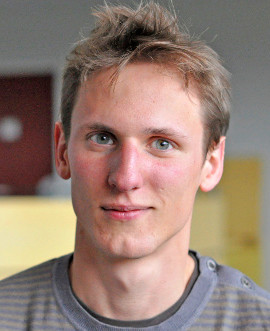
\includegraphics[width=2.4cm]{img/ID_ochurlaud}}; 
			\end{scope}
		\end{tikzpicture}
		\vfill
		~
	\end{minipage}
	\begin{minipage}[c][4cm]{5.5cm}
		\textbf{Olivier CHURLAUD}

		\begin{itemize}[itemsep=0.5ex,leftmargin=3ex]
			\footnotesize
			\item[\bfseries @] \url{olivier@churlaud.com}
			\item[\bfseries \color{blue} in] {\scriptsize\url{ fr.linkedin.com/in/olivierchurlaud/}}
			\item[\Telefon] +49 (0)157 52931348
			\item[\Letter] 12, place du grand four \\
			79 370 MOUGON \\ 
			FRANCE
			\item[$\bullet$] né le 07 avril 1992
		\end{itemize}
	\end{minipage}
	\begin{minipage}[c][4cm]{10cm}
		\begin{minipage}[c]{7.10cm}
			
\includegraphics[width=6.5cm]{img/ecl}
		\end{minipage}
		\hfill
		\begin{minipage}[c]{2.5cm}
			
\includegraphics[width=2.1cm]{img/tuberlin}
		\end{minipage}
		
		\vfill
		
		\centering
		{
			\setlength{\parskip}{10pt plus 1pt minus 1pt}
			{\LARGE \'Elève Ingénieur}
			
			{\Large Spécialité traitement du signal et de l'information}
		}
	\end{minipage}
\end{minipage}

\vfill
\begin{minipage}{\linewidth}
	~
	\hfill
	\begin{minipage}{\scale\linewidth}
	~
		\section*{\'Etudes}
		\begin{tabular}{p{\datescale\linewidth} P{\descripscale\linewidth}}
			\itemcv{2014 -- 2016}{TU Berlin : Master Elektrotechnik}
			\itemcv{2012 -- 2016}{École Centrale de Lyon : Préparation du diplôme d'ingénieur généraliste}
			\itemcv{2010 -- 2012}{Classe préparatoire Maths-Physiques (MP) au Lycée Pierre de Fermat de Toulouse (31)}
		\end{tabular}
		
		\section*{Expériences}
		\subsection*{Direction de projets}
		
		\begin{tabular}{p{\datescale\linewidth} P{\descripscale\linewidth}}
			\itemcv{2013 -- 2014}{
				\textbf{Projet de Recherche : Conception et création d'un module de transmission WPAN-WLAN} \\
				Collaboration avec le laboratoire INL (Lyon) \\
				\textit{Programmation C -- Conception KICAD -- Microcontrôleurs Microchip}
			}
			\itemcv{2012 -- 2013}{
				\textbf{Président de l'association ECLAIR} (association loi 1901 gérant l'informatique et le réseau de l'École Centrale de Lyon : 700 utilisateurs) : Mise en place d'un Cloud, Conception d'un méta-site interne pour les élèves et anciens élèves
			}
			\itemcv{~}{
				\textbf{Projet d’Étude : Création d'un outil de mesure des champs magnétiques de basse fréquence} \\
				Collaboration avec le Laboratoire Ampère (Lyon) \\
				\textit{Programmation MATLAB -- Mise en œuvre d'un magnétomètre}
			}
			\itemcv{2009 -- 2010}{
				\textbf{Projet de recherche en physique des particules en partenariat avec le CERN et l'IN2P3} \\
				Projet soutenu aux Olympiades de Physiques (1\ier prix), aux Faites de la Science (1\ier prix) \\
				\textit{Expérimentations -- Vulgarisation -- Conception d'un jeu de plateau sur le thème du LHC}
			}
			\itemcv{2008 -- 2009}{
				\textbf{Projet d'Atelier d'écriture en partenariat avec l'OuLiPo} (Ouvroir de Littérature Potentielle : groupement	d'écrivains qui travaille en se choisissant des contraintes de fond et de forme)
			}
		\end{tabular}
		
		\subsection*{Expériences professionnelles}
		
		\begin{tabular}{p{\datescale\linewidth} P{\descripscale\linewidth}}
			\itemcv{2014}{
				\textbf{Stage d'application : Télécom Bretagne, avec F.P. Andriulli} -- Analyse et développement de techniques et d'outils	expérimentaux et computationnels pour l'imagerie cérébrale par encéphalogramme
			}
			\itemcv{2013}{
				Stage ouvrier : \textbf{SNCF} - maintenance de locomotives BB26000 (Technicentre SNCF Oullins)
			}
			\itemcv{2010 et 2011}{
				Emploi saisonnier : manutention dans une entreprise de déménagement (BIARDEAU SARL, à Niort)
			}
		\end{tabular}

		\section*{Compétences}
		
		\begin{tabular}{p{\datescale\linewidth} P{\descripscale\linewidth}}
			\itemcv{Management}{Chef de projet, coordination d'équipes, lien entre administration et équipe}
			\itemcv{Électronique}{Programmation de microcontrôleurs Microchip, cartes électroniques de communication WPAN/WLAN}
			\itemcv{Informatique}{
				Programmation, Machine Learning --
				\textbf{Administration système et réseaux} Linux, Bridging, VLAN, Virtualisation KVM, Apache2 -- \textbf{Programme} MATLAB, C/C++, MySQL, Python, \LaTeX
			}
			\itemcv{Langues}{
				\textbf{Anglais} (Lu, écrit, parlé : TOEFL 613pts) \\
				\textbf{Allemand} (Lu, écrit, parlé : Certificat de niveau B2 en allemand en 2014 {\scriptsize(Système de notation Européen)})
			}
			\itemcv{Autres}{Permis B}
		\end{tabular}
		
		\section*{Centres d’intérêt}
		
		\begin{tabular}{p{\datescale\linewidth} P{\descripscale\linewidth}}
			\itemcv{Culturel}{Littérature : littérature classique du XIX-XXe siècle et Nouveau Roman}
			\itemcv{~}{Musique, Cinéma : Cinéma d'auteur et des années 40-50}
			\itemcv{Sport}{Sports de montagne : ski, escalade, randonnée}
	\end{tabular}
	\end{minipage}
\end{minipage}
\vfill
\end{document}